\documentclass[fleqn,10pt,  amsmath,amssymb,aps]{wlscirep}
\usepackage[utf8]{inputenc}
\usepackage[T1]{fontenc}
\usepackage{hyperref}
\usepackage{cleveref}

\title{Information dynamics in neuromorphic nanowire networks}

\author[1,*]{Alice Author}
\author[2]{Bob Author}
\author[1,2,+]{Christine Author}
\author[2,+]{Derek Author}
\affil[1]{Affiliation, department, city, postcode, country}
\affil[2]{Affiliation, department, city, postcode, country}

\affil[*]{corresponding.author@email.example}

\affil[+]{these authors contributed equally to this work}

%\keywords{Keyword1, Keyword2, Keyword3}

\begin{abstract}
Example Abstract. Abstract must not include subheadings or citations. Example Abstract. Abstract must not include subheadings or citations. Example Abstract. Abstract must not include subheadings or citations. Example Abstract. Abstract must not include subheadings or citations. Example Abstract. Abstract must not include subheadings or citations. Example Abstract. Abstract must not include subheadings or citations. Example Abstract. Abstract must not include subheadings or citations. Example Abstract. Abstract must not include subheadings or citations.
\end{abstract}
\begin{document}

\flushbottom
\maketitle
% * <john.hammersley@gmail.com> 2015-02-09T12:07:31.197Z:
%
%  Click the title above to edit the author information and abstract
%
\thispagestyle{empty}

\noindent Please note: Abbreviations should be introduced at the first mention in the main text – no abbreviations lists. Suggested structure of main text (not enforced) is provided below.

\section*{Introduction}

The Introduction section, of referenced text expands on the background of the work (some overlap with the Abstract is acceptable). The introduction should not include subheadings.

\clearpage

\textbf{General questions about result part}

\begin{itemize}
	\item Do we need the current flux vs node centrality? (basically a straight line) [Nah. Just state node current increases linearly with centrality.]
	\item Do we need communicability? Since COMM = $\sum G^k$ in my definition.	[Probably not - we have more than enough results and I don't think this adds anything.]
	\item  For the coloring of TE scatter, ON time might be a more straight forward scheme, e.g. the color-way in AIS vs centrality plot. [Yes, to be consistent and especially if we don't include common. Also, this will combine fig 6 \& 7 into one plot, which is better.]
	\item How to name different regimes of activation and what will be the time points to distinguish them. [How about: pre-activation, activation and post-activation?]
	\item What will be the best incentive for different initial states in benchmarking. (As far as I know, most of the reservoir computing realizations are based on homogeneous or randomly generated initial states. This pre-activated way might be a good alternative.)[Let's ask Joe - he and Mac and Mike were looking into this with ANNs as there is now some literature on pre-activating ANNs (but not ESNs/RC networks ).]
	\item The word usage of node-edge and wire-junction. (In the context of graph/network, seems like node and edge are more understandable. But when talking about ON/OFF and filament states, I feel like junction makes more sense. Should we just use one pair of representation in the paper?) [Yes we should try and be consistent. For this study, we don't need to use filament, but I think we can interchangably use node/wire and edge/junction, and junction state.]
\end{itemize}


\clearpage
\section*{Results}

\textbf{Include some explanation about the network's activation under DC signal. And the fact most of the analysis are done with snapshots.}

\textbf{Talk about the sim settings and the network being used.}

As the network is being activated, junction filament states will grow faster at more ``central" positions. A winner-takes-all current path \textbf{Cite Dublin paper} will form at the most central nodes first, then branch out to the rest of the network. At a specific time $t$, current-flow betweenness centrality of junctions can be determined by Eq. \ref{eq:ebc}. Junctions with higher centrality are more likely to exhibit higher voltage and filament state. Voltage ($\vec{V_e}$) and filament state ($\vec{\lambda}$) are strongly coupled on the junctions; higher voltage on a junction will lead to faster growth of its filament state. In return, a higher filament state means the junction will have a higher conductance (\textbf{refer to equation here}), and an increased chance to reach higher voltage.

% Among all sorts of metrics, voltage distribution on nodes $\vec{V_n}$ and on edges $\vec{V_e}$ would be the most interesting ones since the change rate of conductances exhibited by edges are determined by $\vec{V_e}$. Meanwhile changes of conductance at edges will lead to a redistribution of voltage across the voltage.

\paragraph{Filament state}

The absolute values of filament states $|\vec{\lambda}(t)|$ as a function of edge current-flow betweenness centrality are plotted on Fig. \ref{fig:v_lam_cent}, colored by corresponding conductance. The plot shows that junctions at more central positions will have faster filament growth. **  \textbf{[Alon - this is repeating]} The color spectrum on the plot demonstrates the conductance transition of junctions based on their filament states.\textbf{JOEL: could refer to this as an increase in tunnelling conductance or transition to ballistic conductance.} High centrality junctions have significantly higher conductance since their filament states are greater than the threshold [ \textbf{Alon - do you mention threshold earlier? talk about threshold or ref]}. Consequently, these junctions are preferred during formation of the first current path.

\paragraph{Voltage distribution} 

Voltage distribution on junctions $|\vec{V_e}|(t)$ as a function of centrality is also included in fig. \ref{fig:v_lam_cent}. The data points can be clearly classified into three regimes: The two linear regimes at the left and right ends correspond to the OFF and ON junctions. The transition regime in the middle consists of the junctions whose conductance are in transient between low and high \textbf{[Alon -  wording here doesn't sound right][Ru - I guess still need some suggestions here]}. Within each regime, junctions with higher centrality will have higher voltage. Earlier current paths consist of these higher centrality junctions.

\begin{figure}[h]
	\centering
	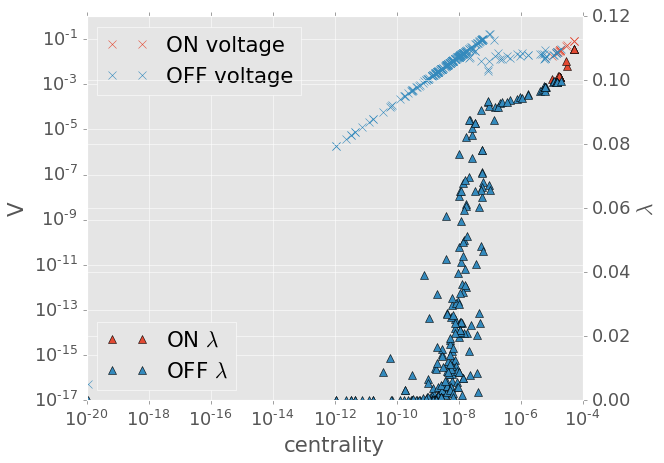
\includegraphics[width=0.5\linewidth]{figure/v_lam_cent}
	\caption{Absolute values of voltage and filament as a function of centrality at T = ?? s. Current path was formed at ??. The data points are colored based on the junctions' corresponding conductance. \textbf{ASK Zdenka. Maybe junction on time will be a more obvious metric.}}
	\label{fig:v_lam_cent}
\end{figure}

\paragraph{Current flow}
\textbf{Not sure if we have  to keep this}
The cumulative current flow through nanowires shows a linear relationship with node current flow betweenness centrality. 
% fig. \ref{fig:i_cent}.

\begin{figure}[h]
	\centering
	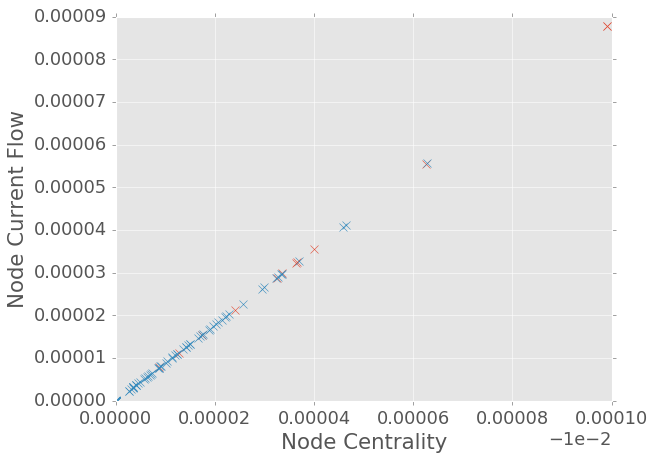
\includegraphics[width=0.5\linewidth]{figure/I_cent}
	\caption{Current flow on a nanowire vs node centrality}
	\label{fig:i_cent}
\end{figure}

\subsection*{Centrality and Functionality}

\textbf{NOT sure if we want to keep communicability. Since COMM = $\sum G^k$}

\textbf{WORDING HERE as well.} Intuitively one would think certain nodes in the network will have a more important role for specific functionalities \textbf{[Alon - based on what intuition? maybe citation?][Good question, need to think about it ]}. Here analysis of the network's functionality such as communicability and transfer entropy are presented. The results suggest that more central wires (\textbf{Be explicit about more central: higher centrality.}) and junctions have higher importance in information dynamics ...\textbf{MAYBE communicability}.  

The communicability of nodes at $t$ can be calculated based on eq. \ref{eq:ncomm}. At an arbitrary time point during the activation (Right after first current path formation here ), when plotted as a function of current-flow closeness centrality on log-log scale, communicability shows as a close to exponential curve, indicating that the nodes at more central positions are more communicable to the rest of the network as this time point. 

\begin{figure}[h]
	\centering
	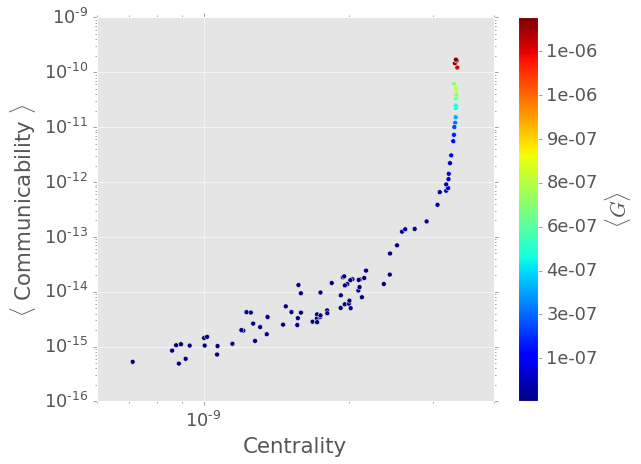
\includegraphics[width=0.5\linewidth]{figure/comm_cent}
	\caption{\textbf{Node communicability vs closeness centrality at $t = 2 s$.} Node communicability is calculated by eq. \ref{eq:ncomm}. Closeness centrality is calculated by eq. \ref{eq:ecc}. The plot is done on log-log scale. As the nodes at more central positions are having much higher communicabilities (and higher conductance). And the other nodes follows a close to linear trend.}
	\label{fig:comm_cent}
\end{figure}

The node closeness centrality also shows an interesting correlation with transfer entropy. For any node in the network, the out-TE is considered as the average transfer entropy measured from the node to its neighbors. Oppositely, the in-TE is defined as the transfer entropy from all neighbors to the node. \textbf{(Have to write equations to define in and out)}. With 50 repetitions of different source/target node pairings (while the graphical distance in between is kept constant), TE averaged across the whole time-series shows a close-to-linear relationship with centrality on a semi-logy scale in Fig. \ref{fig:in_te}. Centrality here is calculated at $t = 0\,$s, and therefore reflects the influence of the structural properties of the network (as all junctions have equal weights at $t = 0$s). Nodes at more central positions have the potential to send out and take in more information and exhibit richer dynamics (\textbf{might have to explain about "richer"}).

Fig. \ref{fig:TE_cent_act} shows the in-TE vs closeness centrality around the time of formation of winner-takes-all current path ($T = ..$ here). On a semi-logy scale, the high centrality nodes exhibit high TE and communicability. At $T = ..$, these nodes are connected to junctions that are already turned ON. On the other hand, the group at the left of the figure consists of low centrality nodes \textbf{[Alon - i feel like a sentence is missing explaining this, and connecting to the next sentence]}. Within this regime, nodes with higher centralities are more likely to have larger TE. The transition from low TE to high TE with respect to centrality increase validates the analysis in fig. \ref{fig:in_te}.

\textbf{Talk about graph metrics, ON/OFF in INTRO}

Furthermore, fig. \ref{fig:EC_AIS} suggests that junctions with higher betweenness centralities tend to have lower active information storage (AIS) and will be turned on relatively earlier. This kind of behavior is consistent with our expectation - junctions at more central locations tend to get higher voltage, meaning filament growth will be faster and a high-conductance state may be reached earlier. Rapid filament growth and increase of conductance leads to stronger information dynamics on central junctions. \textbf{(Fast voltage distribution change as well.)} Thus their future states are less predictable with their own history, which means the AIS will be lower \textbf{[Alon - this sentence needs to be clarified] cite Joe here}.

\begin{figure}[h]
	\centering
	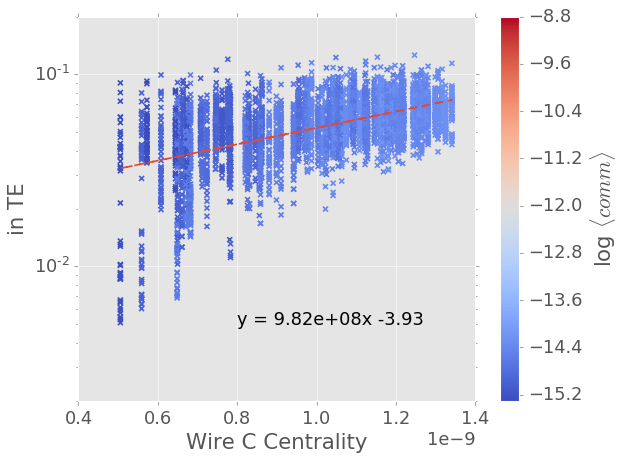
\includegraphics[width=0.5\linewidth]{figure/in_TE}
	\caption{\textbf{Might not need color here. Node in-TE as a function of centrality. (Out TE in  supplement)} 50 repetitions with different source-drain pairings on the same 100 nw network are plotted. Each data point represent one junction in one repetition. TE is averaged across the whole time-series. Node centrality is calculated based on the current-flow closeness algorithm at $t = 0$. Communicability is calculated by Eq \textbf{equation} at $t = 0$ as well. All the source-drain pairings are controlled to have same graphical distance. Identical Mackey-Glass signals are applied to these simulations to activate the network. Each data point on the plot represent one node in one simulation. A close to linear correlation between TE and centrality can be determined from the plot, which means nodes with higher centralities tend to have richer dynamics for taking in and sending out information.
	\textbf{Intrinsic property of the network that does not have any dynamics. We have structural information here.}}
	\label{fig:in_te}
\end{figure}

\begin{figure}[h]
	\centering
	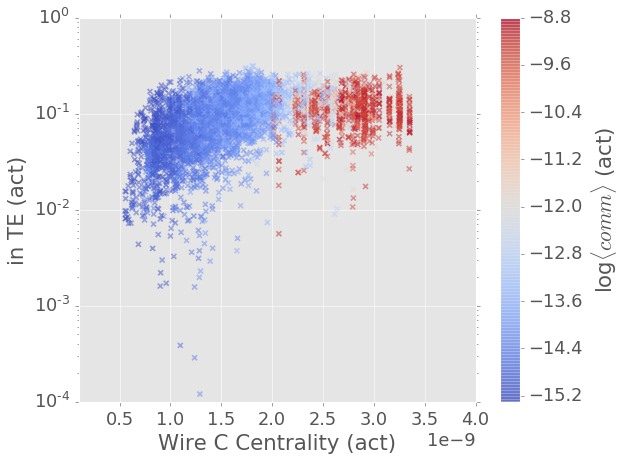
\includegraphics[width=0.5\linewidth]{figure/TE_cent_act}
	\caption{\textbf{In-TE vs closeness centrality around activation.} The same activation test is done as fig. \ref{fig:in_te}.	TE is averaged in a $0.2s$ window right before the activation (mainly to cancel out the randomness). Centrality is measured at the current path formation time.}
	\label{fig:TE_cent_act}
\end{figure}

\begin{figure}[h]
	\centering
	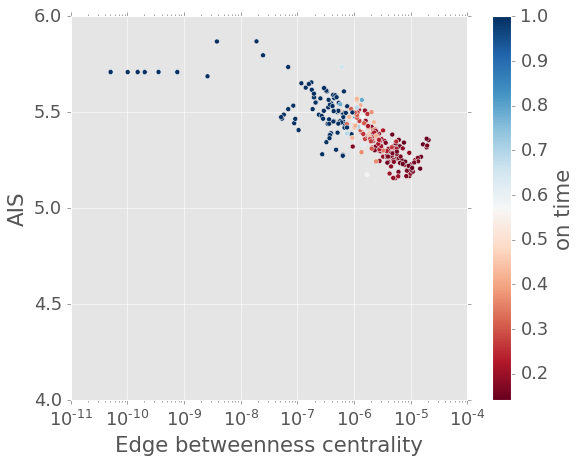
\includegraphics[width=0.5\linewidth]{figure/EC_AIS.png}
	\caption{Active information storage of junctions as function of betweenness centrality.}
	\label{fig:EC_AIS}
\end{figure}




\subsection*{Time-series analysis}

\begin{figure}
	\centering
	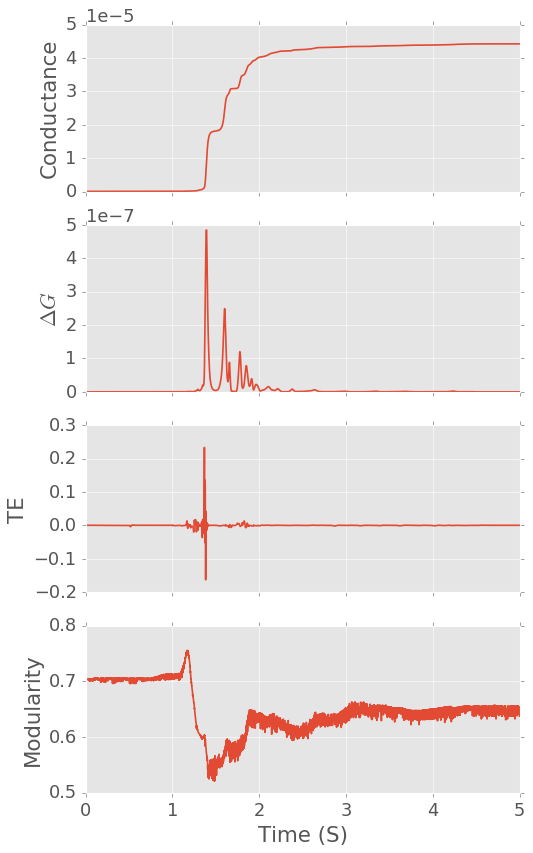
\includegraphics[width=0.5\linewidth]{figure/time_series}
	\caption{\textbf{Time series data for network measures.} The dashed vertical green line represents the 			time of first current path formation.
			\newline (a) Collective conductance of network as a function of time. The collective conductance started increasing when the first junction is turned on. The growth will slow down after the first current path is formed.
			\newline (b) The time derivative of conductance. The derivative is calculated using second order accurate central differences on the collective conductance time series data. The growth regime of conductance shows a great correspondence of $\Delta G$'s spikes.
			\newline (c) Transfer entropy as a function of time. The transfer entropy time series data here is calculated with the Kraskov estimator and averaged across the network. A moving average with window size of 100 is applied to smooth the curve. Transfer entropy in the activation period is significantly higher than the rest.
			\newline (d) Modularity as a function of time. The weighted modularity of network is calculated by Louvain method(Eq. \ref{eq:mod}) As the network evolves, modularity will first increase as high conductance junctions are spread across the network and having their own communities. With the formation of the first current path, the modularity will have a significant drop since these isolating communities are connected. Then the modularity will keep having such fluctuations with smaller scales as more junctions are turned on and forming new current paths.
			\textbf{Gaussian -linear inter, KSG - nonlinear, sensitive}}
	\label{fig:time_series}
\end{figure}

Time series analysis of the network's activation can be even more intriguing. Fig. \ref{fig:time_series}(a) shows the network's collective conductance (\textbf{maybe network conductance}) time-series. The activation of the network mainly have three regimes - the resting (\textbf{maybe another word} ?ground ?low-conductance) regime, the transition regime and the stable (?equilibrium JOEL ?high-conductance) regime. Key events during the activation coincide with each other as a function of time. 

In the resting regime, all junctions are OFF. Collective conductance of the network remains low. Filament states on junctions start to grow based on their voltage. Increase of conductance will first take place at junctions with higher centralities (voltages). Information flow is high when the signal first applied to the network, but in general at a low level in this regime. The modularity level stays constant since all junctions are at low-conductance state. A peak in modularity will then emerge when several junctions in the network starts to have higher conductances as they are forming "highlands" (\textbf{need proper explanation here}). When more junctions experience conductance increase, modularity starts to drop.

(Refer to \ref{fig:time_series}) The transition regime starts when the first junctions is turned on (\textbf{Here it's the tunneling model so maybe some other wording. Like some switches are exhibiting higher conductance}). Collective conductance of the network starts to increase significantly as the time derivative will have a spike. (\textbf{Connect spikes to formation of pathways??? Have to check. Not sure if a clear connection exists.}) Modularity of the network reaches the bottom level \textbf{wording here}. With more junctions turned ON, the first current path (winner-takes-all) will be formed and the conductance keeps increasing with a lower path. Modularity starts to increase again as the nodes on the current path stands out from the rest of the network. Information flow will increase to a higher scale (A spike in Gaussian data). 

\textbf{Show the regimes on figure.}

The transition regime ends when most junctions are at high-conductance states (the rest are not reachable with this specific source-drain pairing). Collective conductance will be stable at a high level. Information flow will decrease to a lower scale similar to the resting regime. The modularity will also be stable in this regime.

Snapshots of the network in different phases shown in fig. \ref{fig:network_comparison}. Nodes are colored with the sum of inTE and outTE averaged in the last $0.2\,$s time window. Similarly, junctions are colored by the sum of the TE flows in both direction in the last $0.2 s$ time window. (Kraskov estimator is used here.) At $t= 0.5 s$, the whole network is at rest. None of the nodes or junctions are having significant information transfer. When the first current path is formed at $t = 1.465 s$, some nodes and junctions start to have significant information flow, but most flows are happening around the central nodes. When $t = 2.0 s$, the information flow is even stronger as more nodes are having high in and out TEs. Meanwhile, even nodes at peripheral positions are having significant information flow. After the network is in the equilibrium regime for a while ($t = 2.5 s$), the information flows decay as the local TE values are significantly lower than the transition regime.

\begin{figure}[]
	\centering
	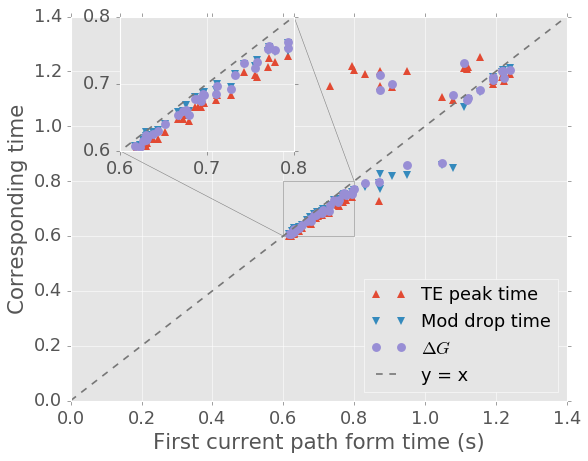
\includegraphics[width=0.5\linewidth]{figure/time_align}
	\caption{\textbf{Key events time as functions of first current path formation time.} 
			The same 100 network is used for 50 simulations with different source-drain pairings. The graphical distances between sources and drains are controlled to be constant. Identical Mackey-Glass signal with random amplitudes ranging between 2-5 V are applied to these simulations. Simulations with higher amplitudes will form current paths earlier. 
			\newline 
			X-axis represents the current path formation time in different simulations. Y-axis represents the corresponding time for key events to take place in these simulations. As shown in this figure, key events such as $\Delta G$ maximum, TE spike (in Gaussian estimation) and modularity drop will happen around the first current path formation time. 
			\newline
			\textbf{Rephrase here} Thus the network will be optimal for information processing and specific task around the transition phase when the first current path is forming and the network is turning on. }
	\label{fig:time_align}
\end{figure}

\begin{figure*}[]
	\centering
	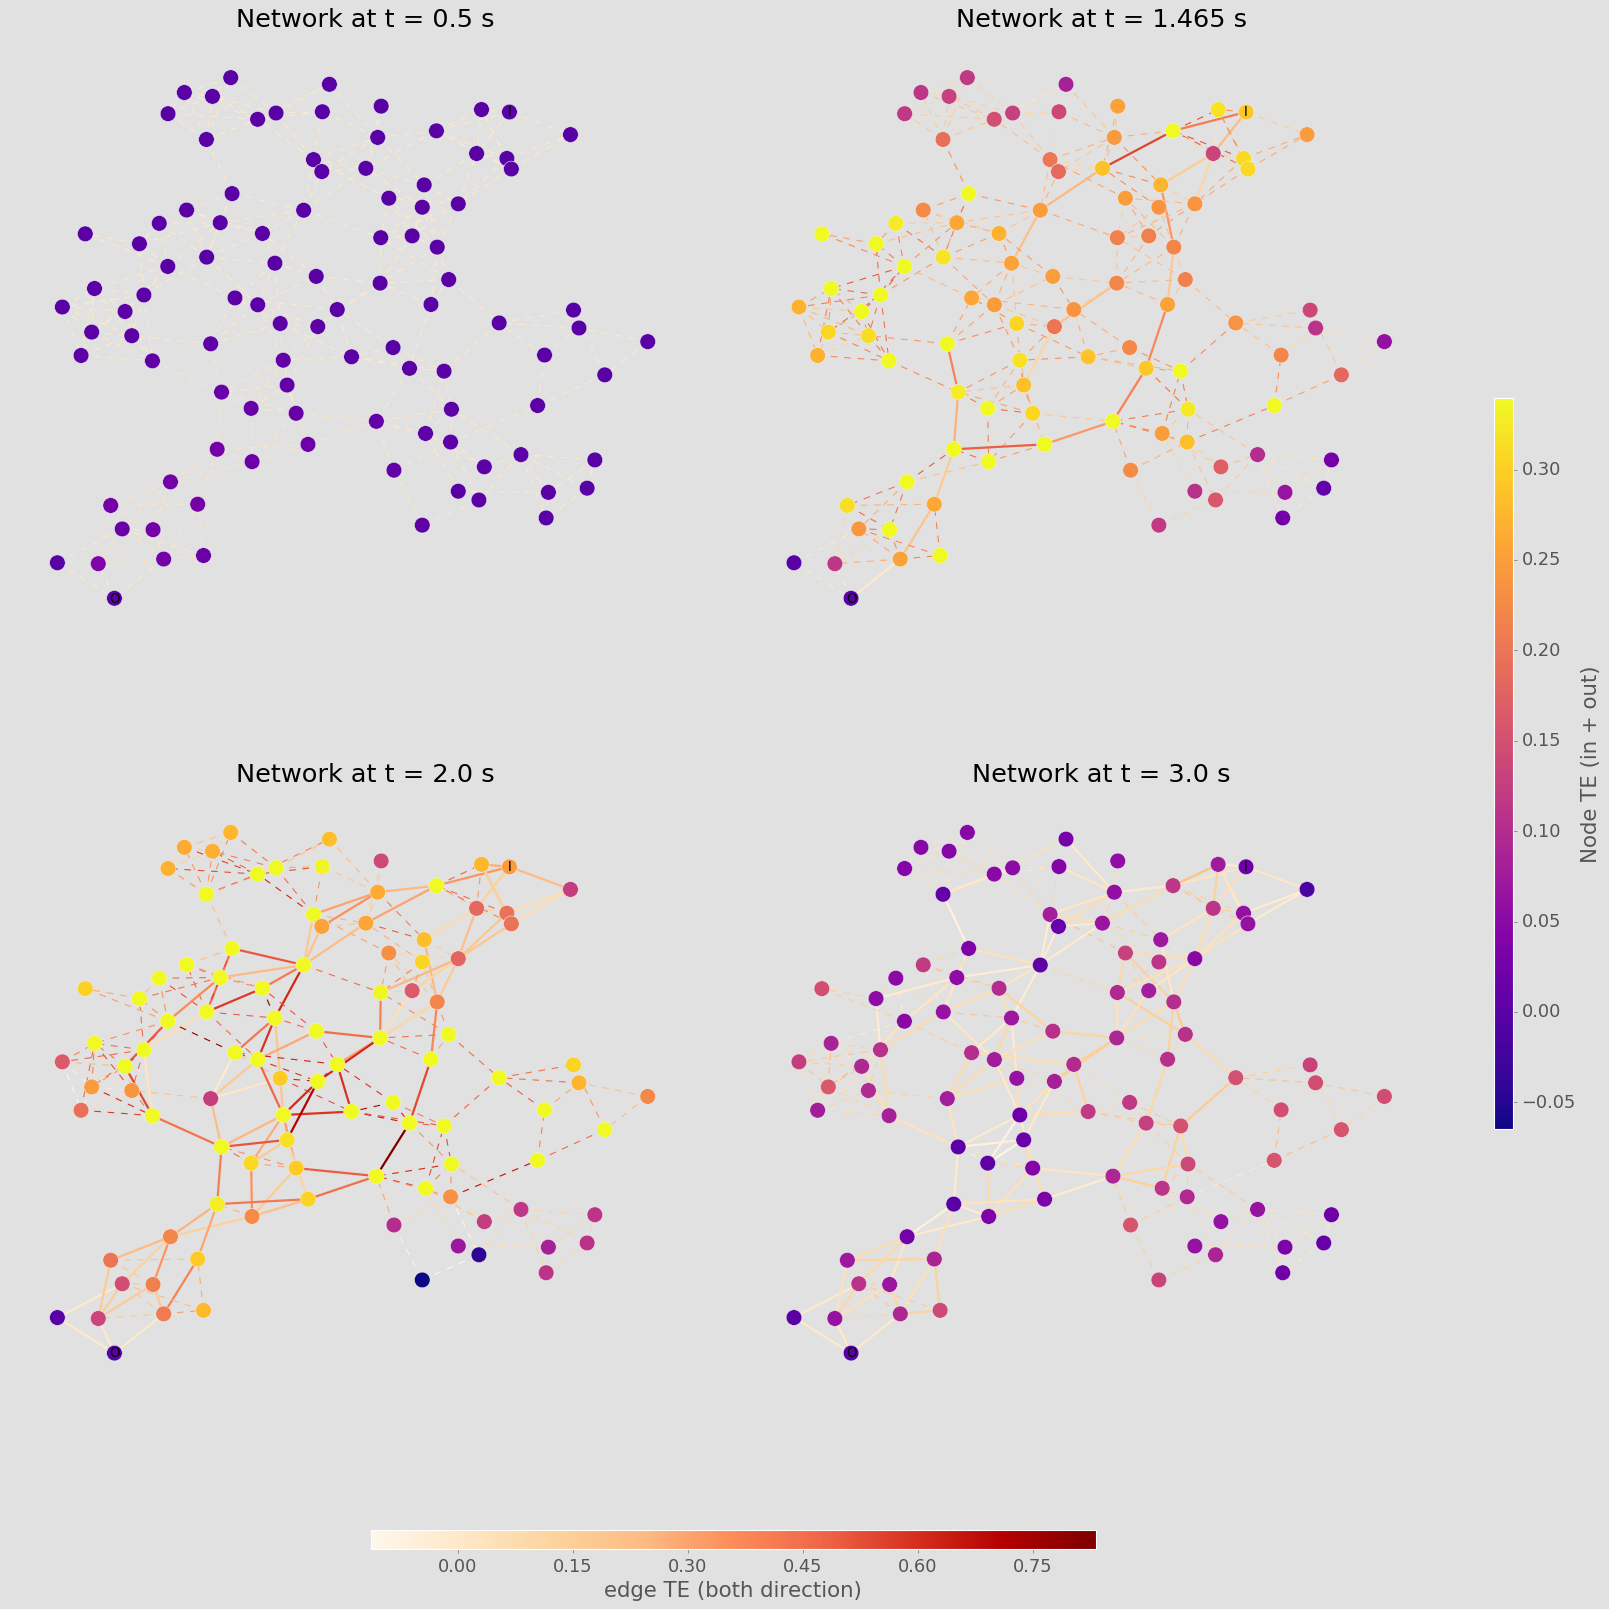
\includegraphics[width = 0.8\paperwidth]{figure/time_network_comparison}
	\caption{\textbf{Network information flow snapshots at different time points.}
			Snapshots of the network are taken at time points before activation ($t = 0.5s$), when the first current path formation ($t=1.465s$), when the network finishes large scale activation ($t = 2s$) and when the network is stable with high collective conductance ($t = 2.5s$).
			Nodes are colored with time-averaged TE flow (inTE + outTE) within the last 0.2 second window using the Kraskov estimator. junctions are colored by the sum of corresponding transfer entropy in both directions. TEs are increasing when the network is being activated and richer dynamics emerge. After the network reaches a stable state (t = 2.5 s), the TEs activities decay as well.}
	\label{fig:network_comparison}
\end{figure*}

A more thorough validation of the hypothesis is done activating the same network with different source-drain pairings. The graphical distance between source and drain in each repetition is controlled to be constant. Identical Mackey-Glass signals with arbitrary amplitude (\textbf{maybe another word like strength/ xxx parameter}) between $2-5\,$V are delivered to the network. The times when the key events take place are recorded and plotted as fig. \ref{fig:time_align}. \textbf{Wording HERE} With the current path formation time on the x-axis, times for other key events line up fairly well. When the amplitude is larger, the first current path will be formed earlier and similar for other events. With amplitude ? greater than 3.5V, the key events line up linearly. With small amplitudes, the activation takes more time and thus more fluctuations in the dynamics (\textbf{fluctuations in dynamics}) are captured. These fluctuations contributes to the outliers in the plot.


% \paragraph{$\Delta G$}

% The conductance time-series of the network reflects the activation stage of the network. Specifically, $\Delta G$ can help identify the avalanche behaviors of the network.


% \paragraph{TE time series}

% The transfer entropy across the whole network is calculated in the same way as before. The average is taken over the whole network the time series to obtain the time series.

% Plotting TE time-series together with $\Delta G$ in the same figure, the spikes of both curves coincide.

% Different amplitude of voltage biases are applied to the network. The activation time and TE peak time in these realizations line-up pretty well.

% \paragraph{Modularity time series}

% Modularity of the network is calculated throughout the activation. The drop of Modularity coincide with $\Delta G$ as well. 


\subsection*{Pre activation task}

\begin{figure*}[]
	\centering
	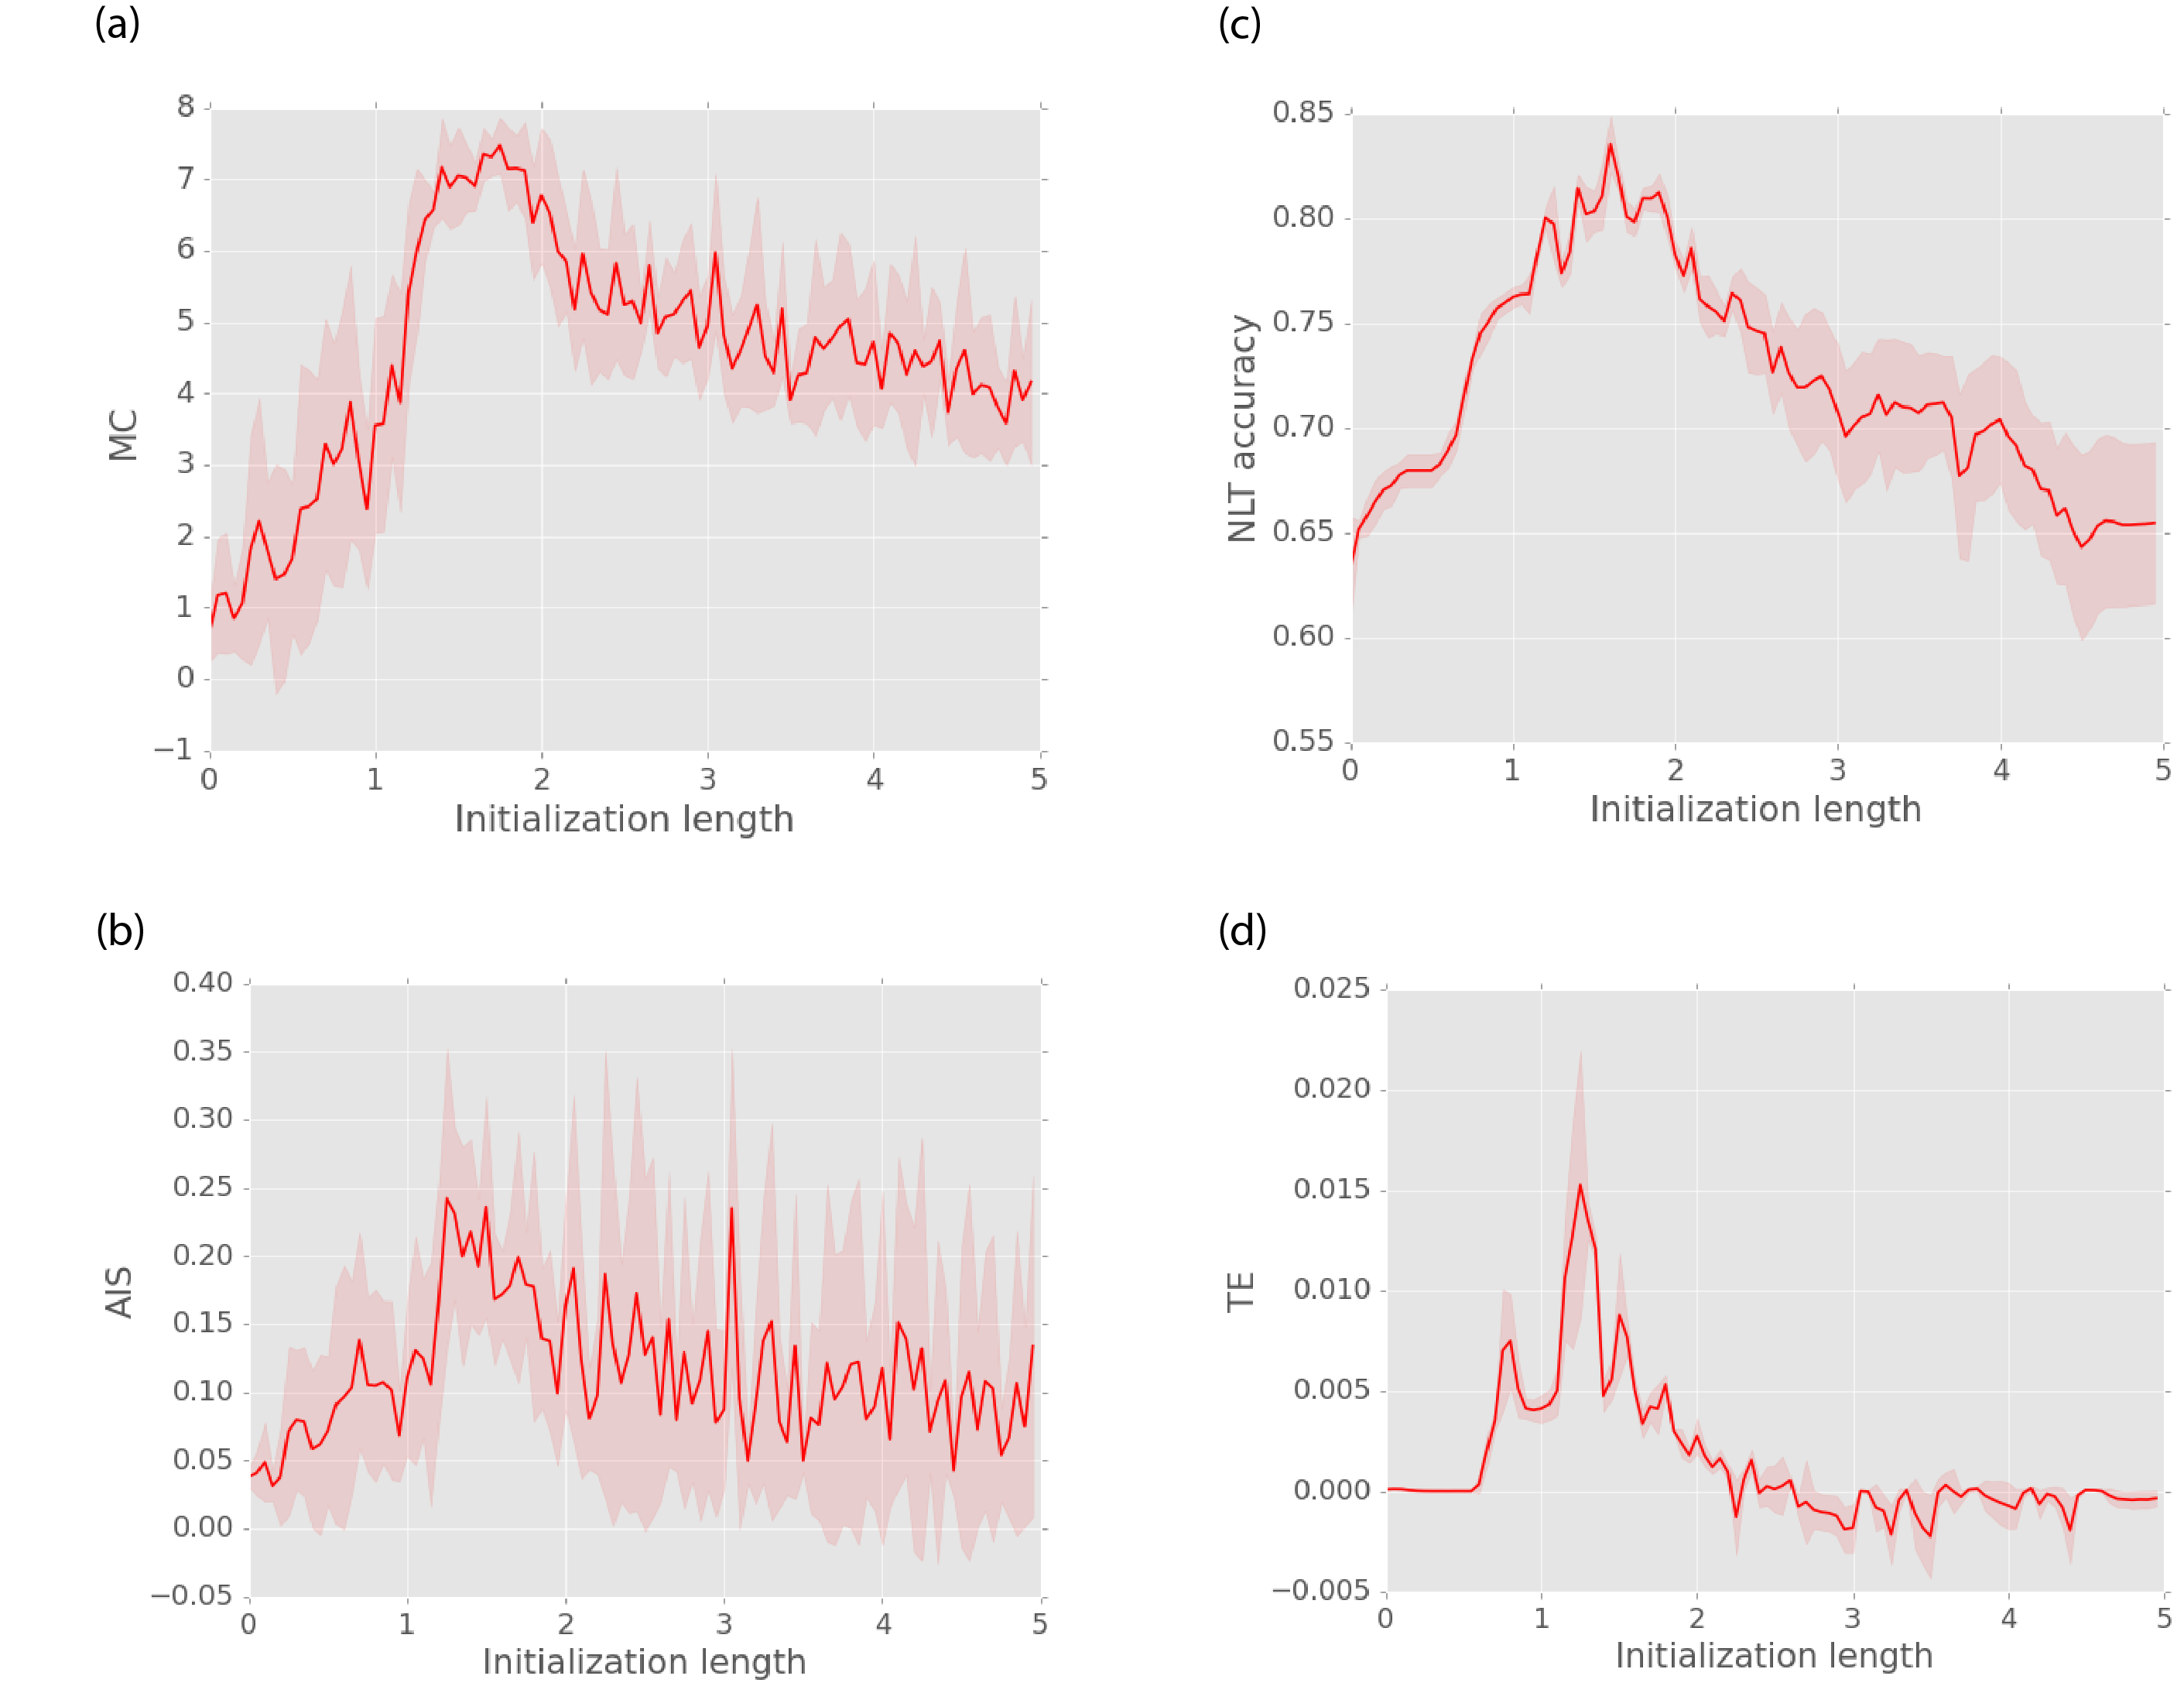
\includegraphics[width=1\linewidth]{figure/benchmark.png}
	\caption{\textbf{Benchmarks of the network with different initial states.} The network's voltage distribution and junction filament states are extracted every 10 time-step during the activation with a Mackey-Glass signal input. Memory capacity/ non-linear transformation tests are then performed accordingly initiating from those pre-activated states. \\
	(a) Memory capacity result with respect to different initial states.\\
	(b) Non-linear transformation performance with respect to different initial states.\\
	(c) Average active information storage of memory capacity tests.\\
	(d) Average transfer entropy of non-linear transformation tests.} 
	\label{fig:benchmark}
\end{figure*}


\textbf{Why we care about different initial states?} 

The same 100-nanowire network is activated with Mackey-Glass signal.(\textbf{Ref here}) The states of the network at different stages during the activation process are extracted and employed as initial states for benchmarks tasks. Memory capacity and non-linear transformation are used to test the network's performance at different activation levels (details in method part). 

Fig. \ref{fig:benchmark} (a) shows the memory capacity of the network with respect to different initial states (\textbf{explain different initial states}). The tests with pre-activation between 1 to 2 seconds are showing significantly better performance compared to the rest. The average active information storages corresponding to these tests are shown in fig. \ref{fig:benchmark} (c). The states with better performance are exhibiting higher active information storage during the tests. Since memory capacity of the network is indicating its capability of short term memory, higher MC coincide with higher AIS is not surprising.

Meanwhile, fig. \ref{fig:benchmark} (b) shows the non-linear transformation performance with different pre-activated states. Similar to the results in MC tests, the states with 1 to 2 seconds of pre-activation perform better than others. However, with roughly around 1.5 seconds of pre-activation, the performance experience a notable drop, which could be caused by the formation of the first current path. As the degree of freedom of voltage distribution is low (\textbf{Need to work on this}) when the first current path is forming. The averaged transfer entropy in non-linear transformation tests is shown in fig. \ref{fig:benchmark} (d). The better performing states show correspondence with higher averaged transfer entropy. Non-linear transformation test requires certainly level of degree of freedom to achieve relatively good performance. According to \textbf{TE equation}, those higher TE tests are exhibiting stronger information dynamics, which is mainly caused by the complexity and uncertainty of voltage distribution. Thus better NLT performance can be explained by higher transfer entropy values in those tests.

\clearpage






\section*{Discussion}

The Discussion should be succinct and must not contain subheadings.

\section*{Methods}

\subsection*{Graph Generalization}

\textbf{Talk about how to map the original nanowire network on to a graph. Cite Zdenka here}.

\begin{figure}[h]
	\centering
	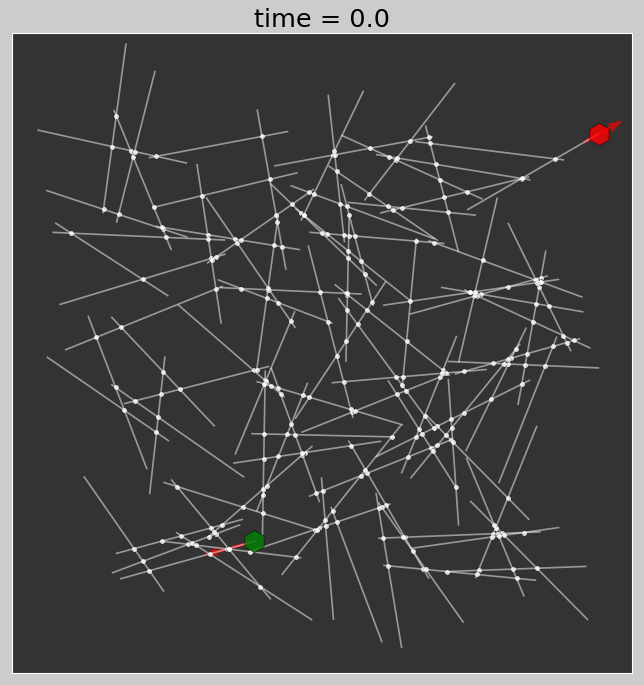
\includegraphics[width=0.8\linewidth]{figure/mpl_plot}
	\caption{}
	\label{fig:mpl_plot}
\end{figure}

\begin{figure}[h]
	\centering
	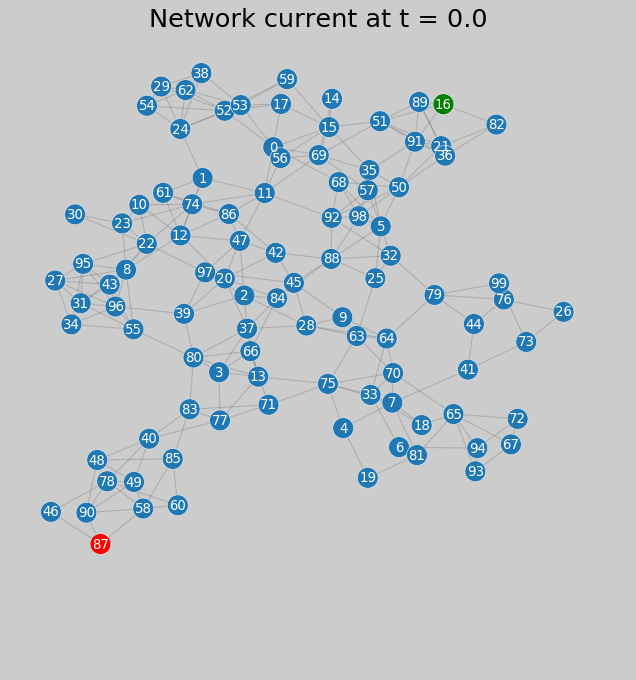
\includegraphics[width=0.8\linewidth]{figure/graph_plot}
	\caption{}
	\label{fig:graph_plot}
\end{figure}

\subsection*{\label{sec:level2} Simulation}
When connected to external voltage biases, nanowire networks behave like traditional electrical networks. Each component in the network obeys Kirchhoff's law. Hence the voltage distribution across the network can be obtained by solving (\cite{Dorfler2018}):

\begin{equation}
{\cal L}^\dagger V = I,
\end{equation}

where $\mathcal{L}^\dagger$ is the expanded graph Laplacian of the network, composed as:

\begin{equation}
	\cal L^\dagger = 
	\left[
	\begin{array}{c|c}
	\cal L&  C\\ 
	\hline
	C^T & \mathbb{0}  
	\end{array}
	\right],
\end{equation}

in which $\cal L$ is the graph Laplacian and $C$ represents the nodes (wires) connected to external electrodes. 

\begin{equation}
{\cal L} = D - W.
\end{equation}

Here $W$ is the weighted adjacency matrix of the network. The weights on edges are determined based on their conductance:
\begin{equation}
	\mathbf W_{ij} = \mathbf A_{ij} G(i,j).
\end{equation}

And $D$ is the weighted degree matrix generated from $W$:
\begin{align}
	d_i = \sum \limits_{k=1}^{N} \mathbf W_{i,k},\\
	\mathbf D = \textbf{diag}(d_i).
\end{align}


\subsection*{Centrality}
Centrality \textbf{Put some reference here} is an important measure that helps understand the fundamental structures and connectivities of networks. Betweenness centrality of nodes and edges in networks can demonstrate .... Meanwhile, closeness centrality of nodes can be used to interpret the ..... \cite{Newman2010}.

A variation of centrality measures based on current flow model proposed by Brandes and Fleischer \cite{Brandes2005} is employed here. As the electrical dynamics in our networks fall in the class of \textbf{random walks} (not sure about here).

The betweenness centrality of a edge in the networks can be determined by:

\begin{equation}
c_{CB}(e) = \frac{\sum \limits_{s \neq t \in V}\tau_{st}(e)}{(n-1)(n-2)},
\label{eq:ebc}
\end{equation}



where $\tau_{st}(e)$ is the current flow through edge $e$ between nodes $s$ and $t$, while $n$ stands for number of nodes in the network.

The closeness centrality of a node in this context is structured in the same way as normal closeness centrality, with distance measured based on effective resistance rather than graphical distance. Therefore it is given by:

\begin{equation}
	c_{CC}(v) = \frac{n-1}{\sum \limits_{v \neq w \in V} R(v,w)}.
	\label{eq:ecc}
\end{equation}
In the context of a unit $st$-current in the network, $R(v,w)$ represents the effective resistance between nodes $v$ and $w$.

\subsection*{Communicability}
Communicability in a network represents .... \cite{Estrada2008}. 

In this work communicability is calculated based on the weighted connections \cite{Crofts2009}. A symmetric matrix $\mathbf M$ is generated to depict the communicability distribution, where $\mathbf M_{ij}$ represents the communicability between nodes $i$ and $j$. Therefore, $\mathbf M$ reads:
\begin{equation}
\mathbf M = \exp{(\mathbf D^{-1/2} \mathbf W \mathbf D^{-1/2})}.
\end{equation} 

The communicability of a node can be defined as how communicable the node is to the rest of the network, which will have the expression as:

\begin{equation}
	m_i = \sum \limits_{k = 1}^N \mathbf M_{ik}, \qquad k \neq i.
	\label{eq:ncomm}
\end{equation}



\subsection*{Modularity}
Modularity is a network metric that ..... \textbf{talk about it here} \cite{Rubinov2009}.

Recent studies in neuro-science demonstrated that modularity plays an important role in .... \textbf{talk about it here} \cite{Godwin2015}. 
 
Modularity ($\mathbf Q^w$) in a weighted network can be calculated by the Louvain method \cite{Blondel2008}:
 
% \begin{equation}
% Q^w = \frac{1}{I^w} \sum \limits_{i,j} \left[W_{ij} - \frac{k_i^w k_j^w}{I^w} \right] \delta(m_i, m_j),
% \end{equation}
\begin{equation}
\mathbf Q^w = \frac{1}{\mathbf D} \sum \limits_{i,j} \left[\mathbf W_{ij} - \frac{d_i d_j}{\mathbf D} \right] \delta(m_i, m_j),
\label{eq:mod}
\end{equation}

in which $w_{i,j}$ is the weight of the edge between nodes $i$ and $j$, $I^w$ represents sum of all weights in the network, $k_i^w$ stands for the weighted degree of node $i$, $m_i$ is the community where node $i$ is located, and $\delta$ is the Kronecker delta function.

\subsection*{Information Dynamics}

Transfer entropy is an effective metric for information dynamics. It explains ..... \textbf{cite Joe here}.

\begin{equation}
T_{Y \rightarrow X} = \sum \limits_{u_n} p(u_n) \log \frac{p(x_{n+1}| x_n^{(k)}, y_n^{(l)})}{p(x_{n+1}|x_n^{(k)})}.
\end{equation}

$n$ is a time index, $u_n$ represents the state transition tuple $(x_{n+1}, x_n^{(k)}, y_n^{(l)})$, $x_n^{(k)}, y_n^{(l)}$ represent the $k$ and $l$ past values of $x$ and $y$ up to and including time $n$. \textbf{rephrase here}.


The transfer entropy across an edge ($e_{i,j}$) is calculated by:
\textbf{Have to write these equations in a better manner.}

\begin{equation}
TE_{i,j} = T_{V_i \rightarrow V_j}
\end{equation}

And therefore the average outward TE and inward TE of a node can be calculated by:

\begin{equation}
\langle TEout_i \rangle = \frac{\sum \limits_{i,j, A_{i,j} \neq 0} TEout}{\text{\# of edges connected to i}}.
\end{equation}


Meanwhile, active information storage was introduced by Lizier et al. (\textbf{cite Joe)} to measure the effect from the past process $\mathbf X$ to the next observation $X_{n+1}$, which is given by:

\begin{align}
	A_X = \lim \limits_{k \rightarrow \infty} A_X (k),\\
	A_X(k) = I(\mathbf X_n^{(k)}; X_{n+1})
	\label{eq:AIS}
\end{align}

The active information storage in context of edge voltage distribution is thus calculated by:

.....

\subsection*{Benchmark}

Regular reservoir computing realizations are typically initialized with homogeneous or randomly generated states. The system then evolves based on specific tasks. \textbf{WHY we want different initial states?}


A nanowire network enters different stages during its activation. Its states at different stages typically have different voltage distribution, unevenly grew filament states and therefore diverse conductance levels. 
In this section the network's states at different activation stages are extracted and used as initial states for benchmarking. Starting from these pre-activated states, memory capacity of the network is measured to estimate the network's ability of reconstructing its short-term memory \textbf{Cite Jaeger}. Non-linear transformation is used to test the network's learning ability \textbf{Cite Kevin}.

A randomly generated time series from uniform distribution in the interval $[-2,2]$ is used as the input signal for memory capacity test. A linear combination of the network's state at $t$ (node voltage) is applied to reconstruct the previous input at $t - k$. $k = 1 ... 100$ are used to investigate different delayed intervals. The $k-$delay memory capacity is defined as:
\begin{equation}
	\text{MC}_k = \dfrac{\text{cov}^2(\mathbf u_{t-k}, \mathbf o_t)}{\sigma^2 (\mathbf u_{t-k}) \sigma^2 (\mathbf o_t)}.
\end{equation}
The generic memory capacity for the network can thus be calculated as:
\begin{equation}
	\text{MC} = \sum \limits_{k=1}^\infty \text{MC}_k.
\end{equation}

The non-linear transformation task makes use of sinusoidal wave as the input signal and try to transfer the signal to other periodic signals in the shape of square or sawtooth. Similar to memory capacity test, linear combinations of the network's states are done to fit the target signal. The accuracy is calculated by $1 - \text{RNMSE}$:
\begin{equation}
	\text{RNMSE} = \sqrt{\dfrac{\sum (\mathbf Y - \mathbf O)^2}{\sum \mathbf O^2}}.
\end{equation}

\bibliography{paper1}\label{paper1}

\noindent LaTeX formats citations and references automatically using the bibliography records in your .bib file, which you can edit via the project menu. Use the cite command for an inline citation, e.g.  \cite{Hao:gidmaps:2014}.

For data citations of datasets uploaded to e.g. \emph{figshare}, please use the \verb|howpublished| option in the bib entry to specify the platform and the link, as in the \verb|Hao:gidmaps:2014| example in the sample bibliography file.

\section*{Acknowledgements (not compulsory)}

Acknowledgements should be brief, and should not include thanks to anonymous referees and editors, or effusive comments. Grant or contribution numbers may be acknowledged.

\section*{Author contributions statement}

Must include all authors, identified by initials, for example:
A.A. conceived the experiment(s),  A.A. and B.A. conducted the experiment(s), C.A. and D.A. analysed the results.  All authors reviewed the manuscript. 

\section*{Additional information}

To include, in this order: \textbf{Accession codes} (where applicable); \textbf{Competing interests} (mandatory statement). 

The corresponding author is responsible for submitting a \href{http://www.nature.com/srep/policies/index.html#competing}{competing interests statement} on behalf of all authors of the paper. This statement must be included in the submitted article file.

Figures and tables can be referenced in LaTeX using the ref command, e.g. Figure \ref{fig:stream} and Table \ref{tab:example}.

\end{document}